\chapter{Current Dynamics and Free Induction Decay}
% \label{chap:conclusion}


\section{Exponential Decay}


\begin{figure}[h!] % можно [t], [b], [p], [h]
    \centering
    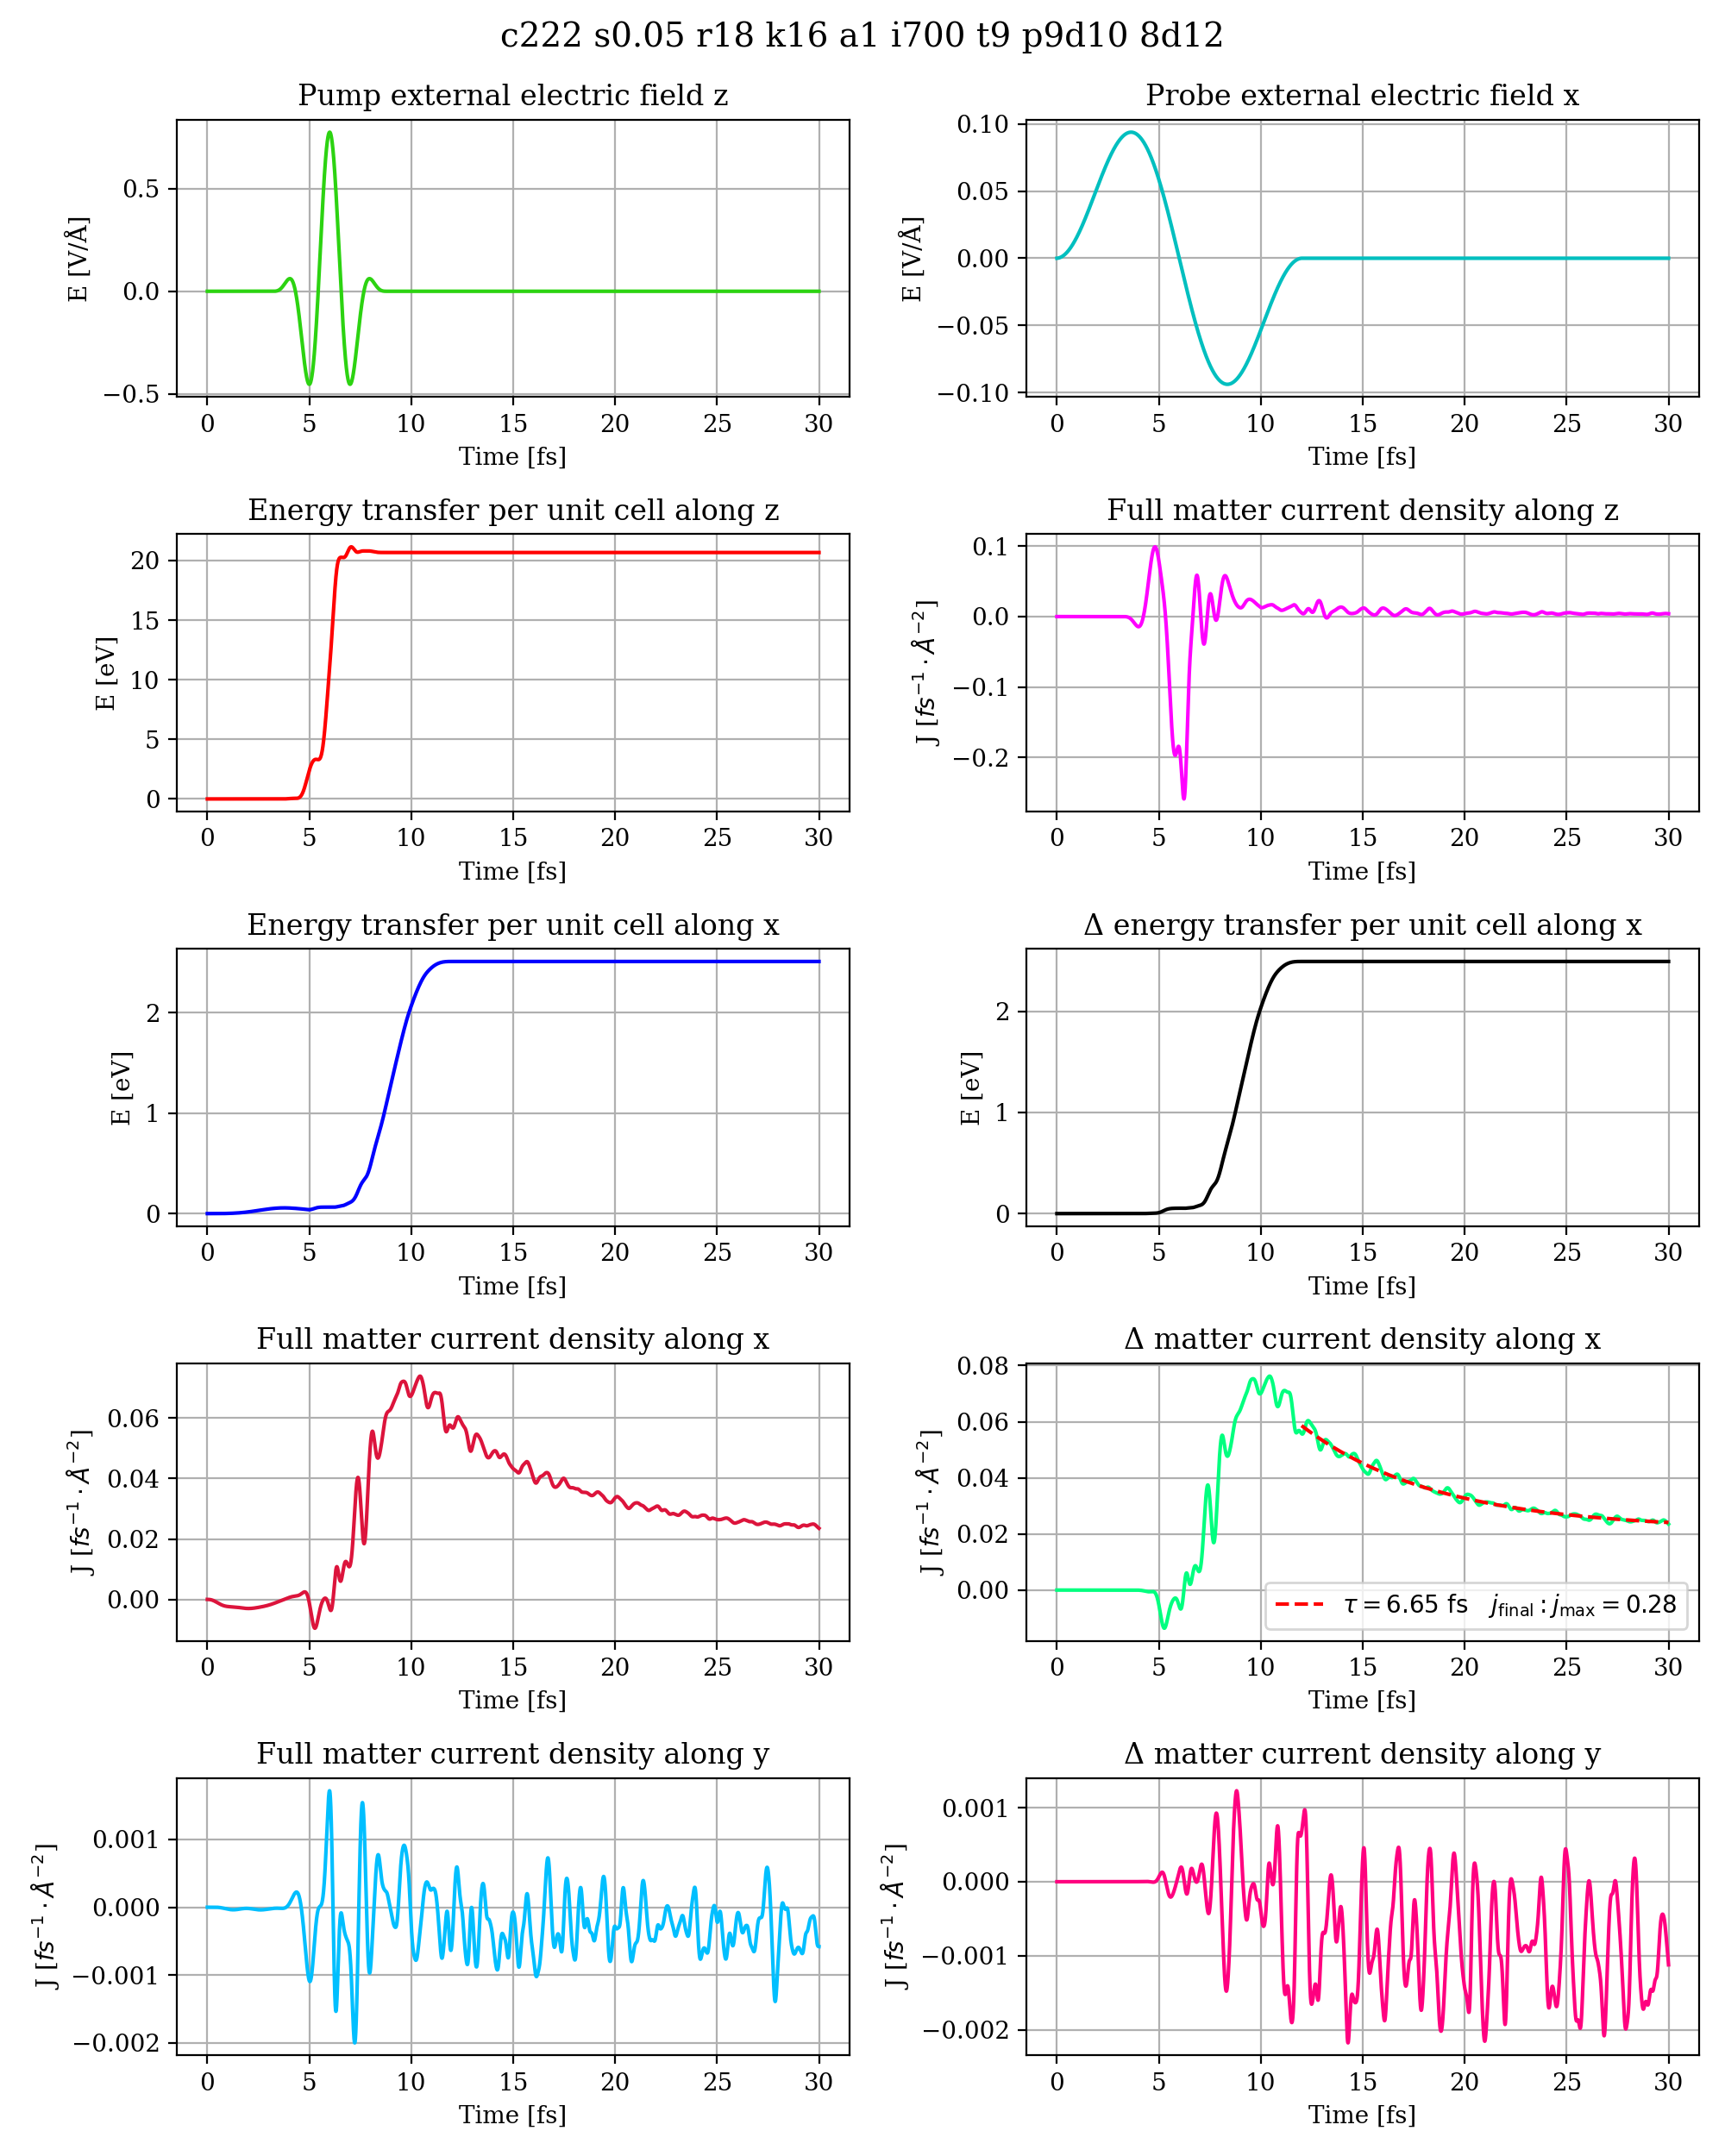
\includegraphics[width=0.68\linewidth]{figures/pump_probe_v1.png} % путь к файлу
    \caption{Energy and current characteristics for different degrees of disorder. Mean energy in the pump pulse is 1.5 eV.}
    \label{fig:myimage}
\end{figure}

The exponential fit works quite well for the dynamics of the current without any electric field. However, Drude model fails. The generalized model needs to be applied. You can start with a simple accounting of the dependence of the relaxation time on the wave vector (found numerically), or try methods used in \cite{PhysRevB.79.115306}.

\begin{figure}[h!] % можно [t], [b], [p], [h]
    \centering
    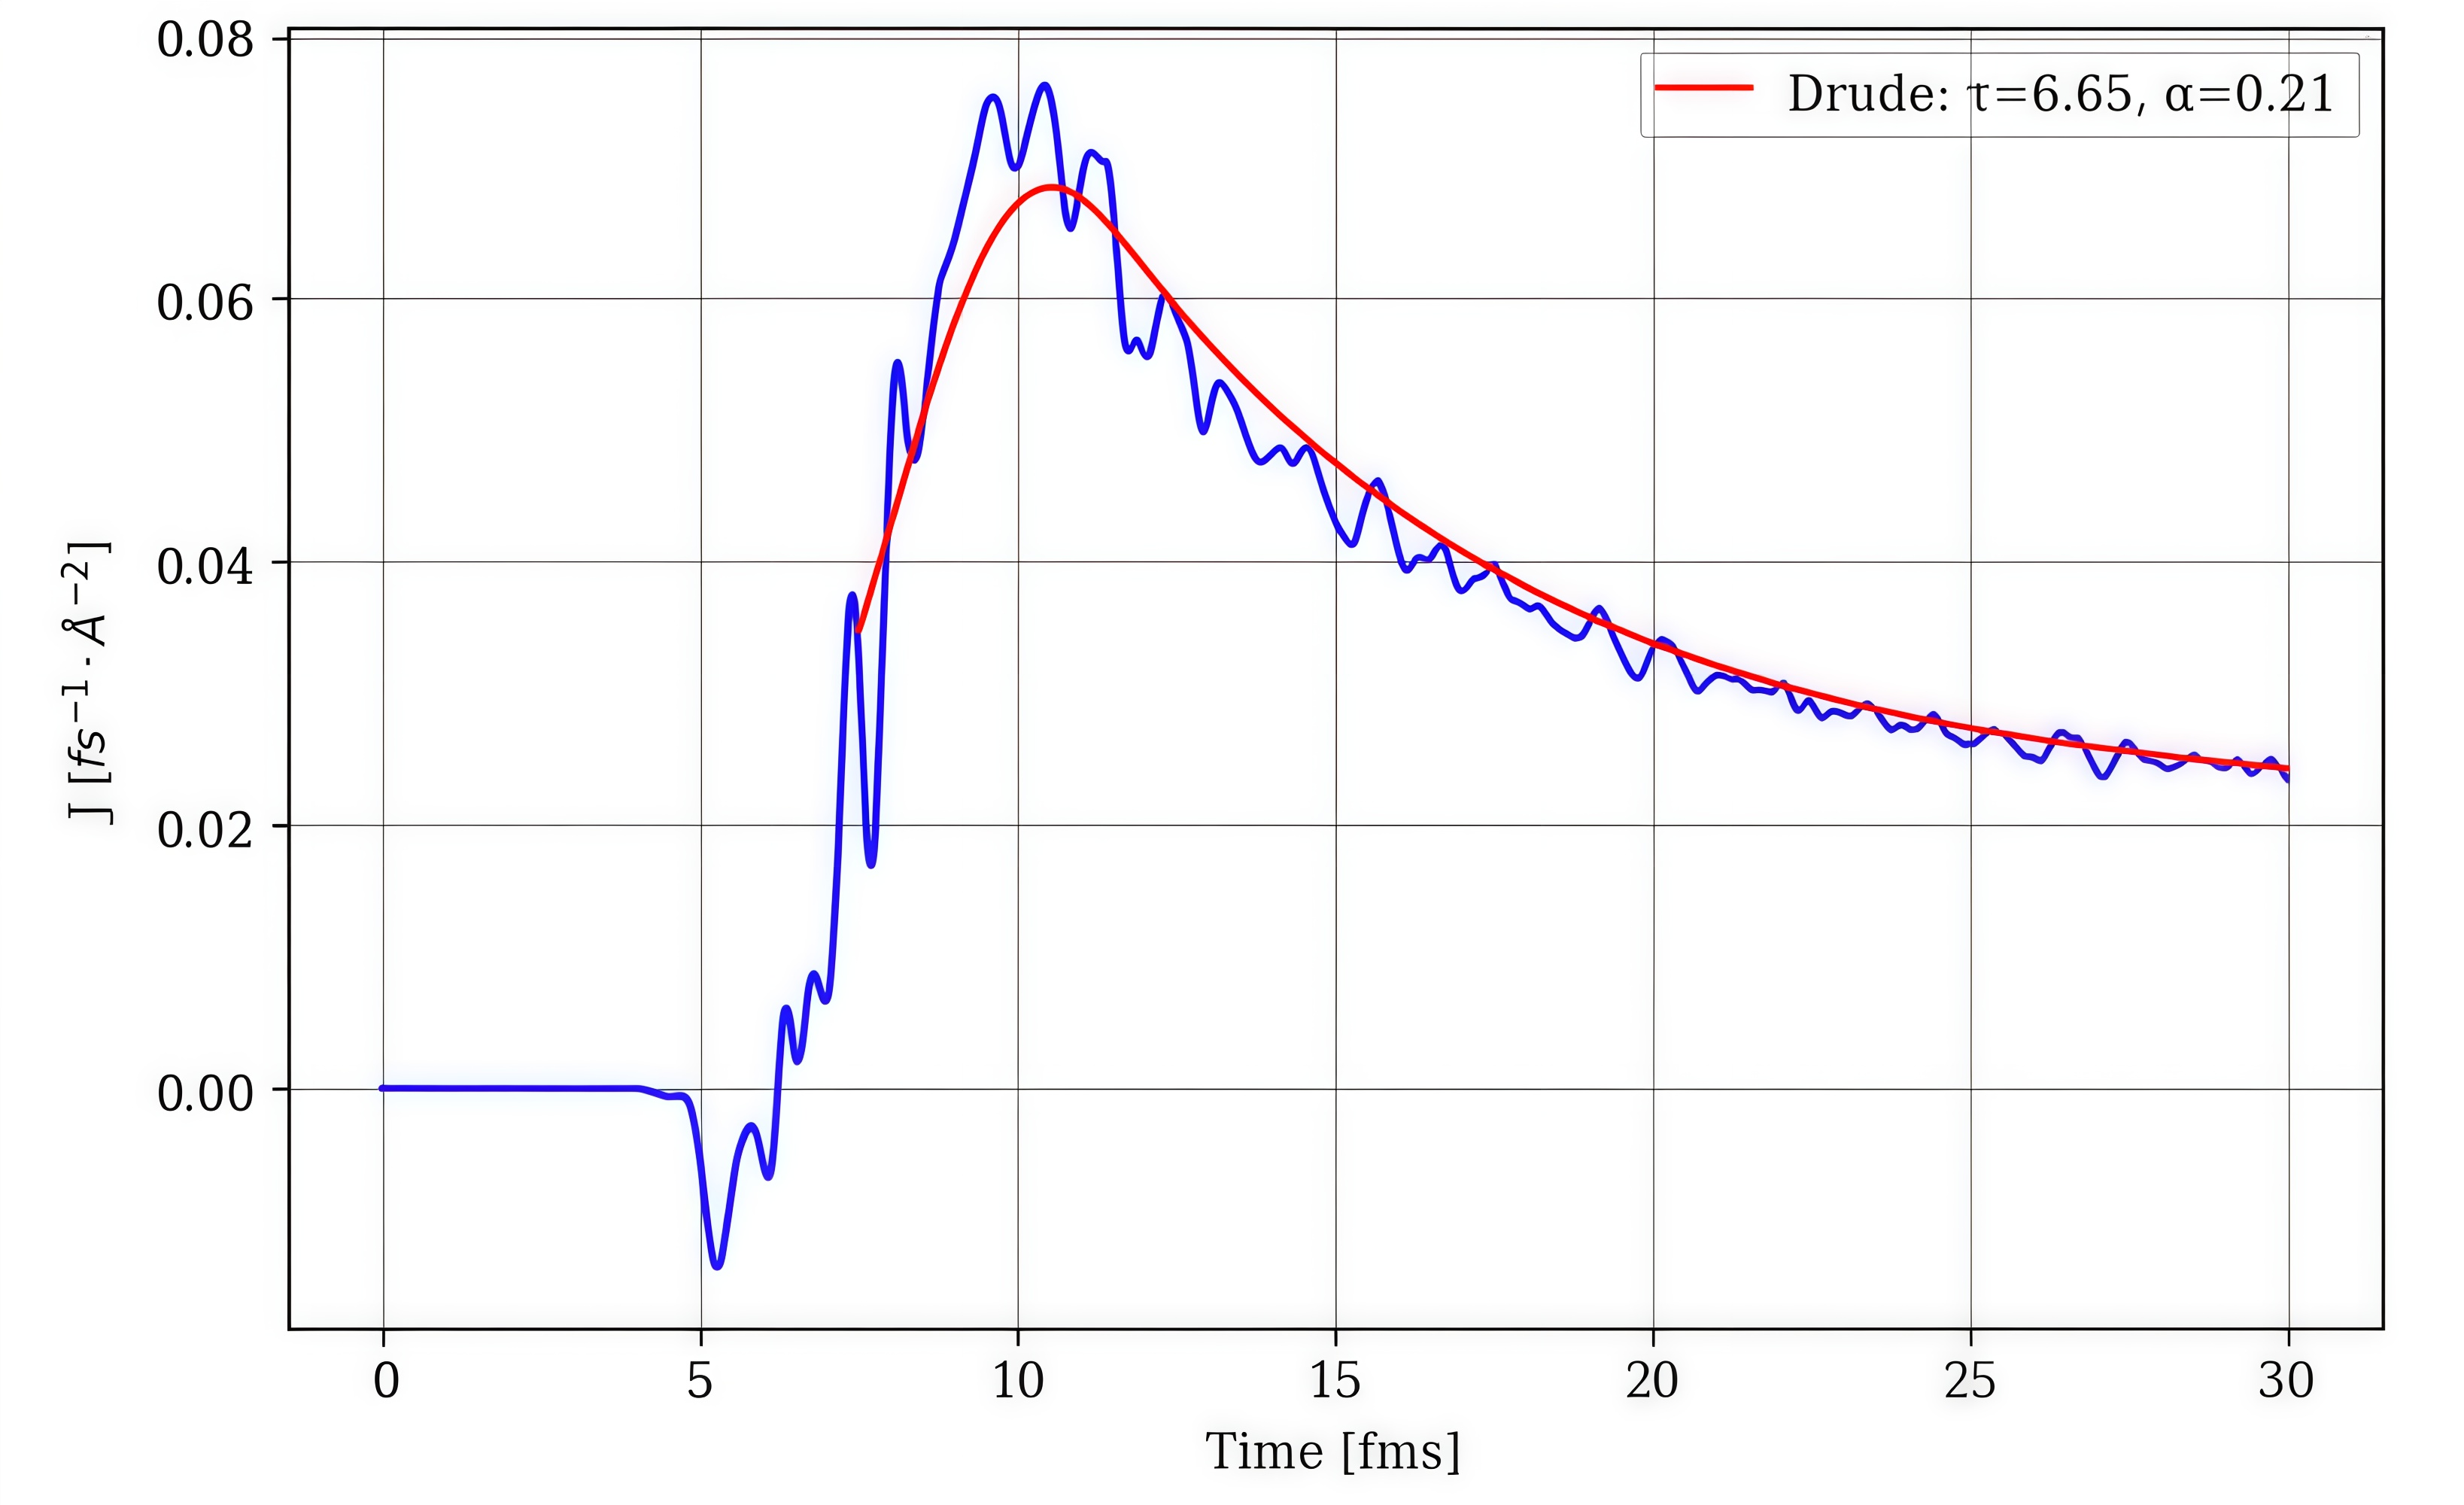
\includegraphics[width=0.8\linewidth]{figures/pump_probe_v1_Drude.png} % путь к файлу
    \caption{Drude model fit.}
    \label{fig:myimage}
\end{figure}

It's also possible to study the attenuation properties by introducing a delay for the test pulse. However, it will be difficult to ensure that it's a half-cycle, since SALMON requires the potential vector to be zero at the beginning and end of the pulse.


\section{Dependence of Relaxation Time on the Wave Vector}

\begin{figure}[h!] % можно [t], [b], [p], [h]
    \centering
    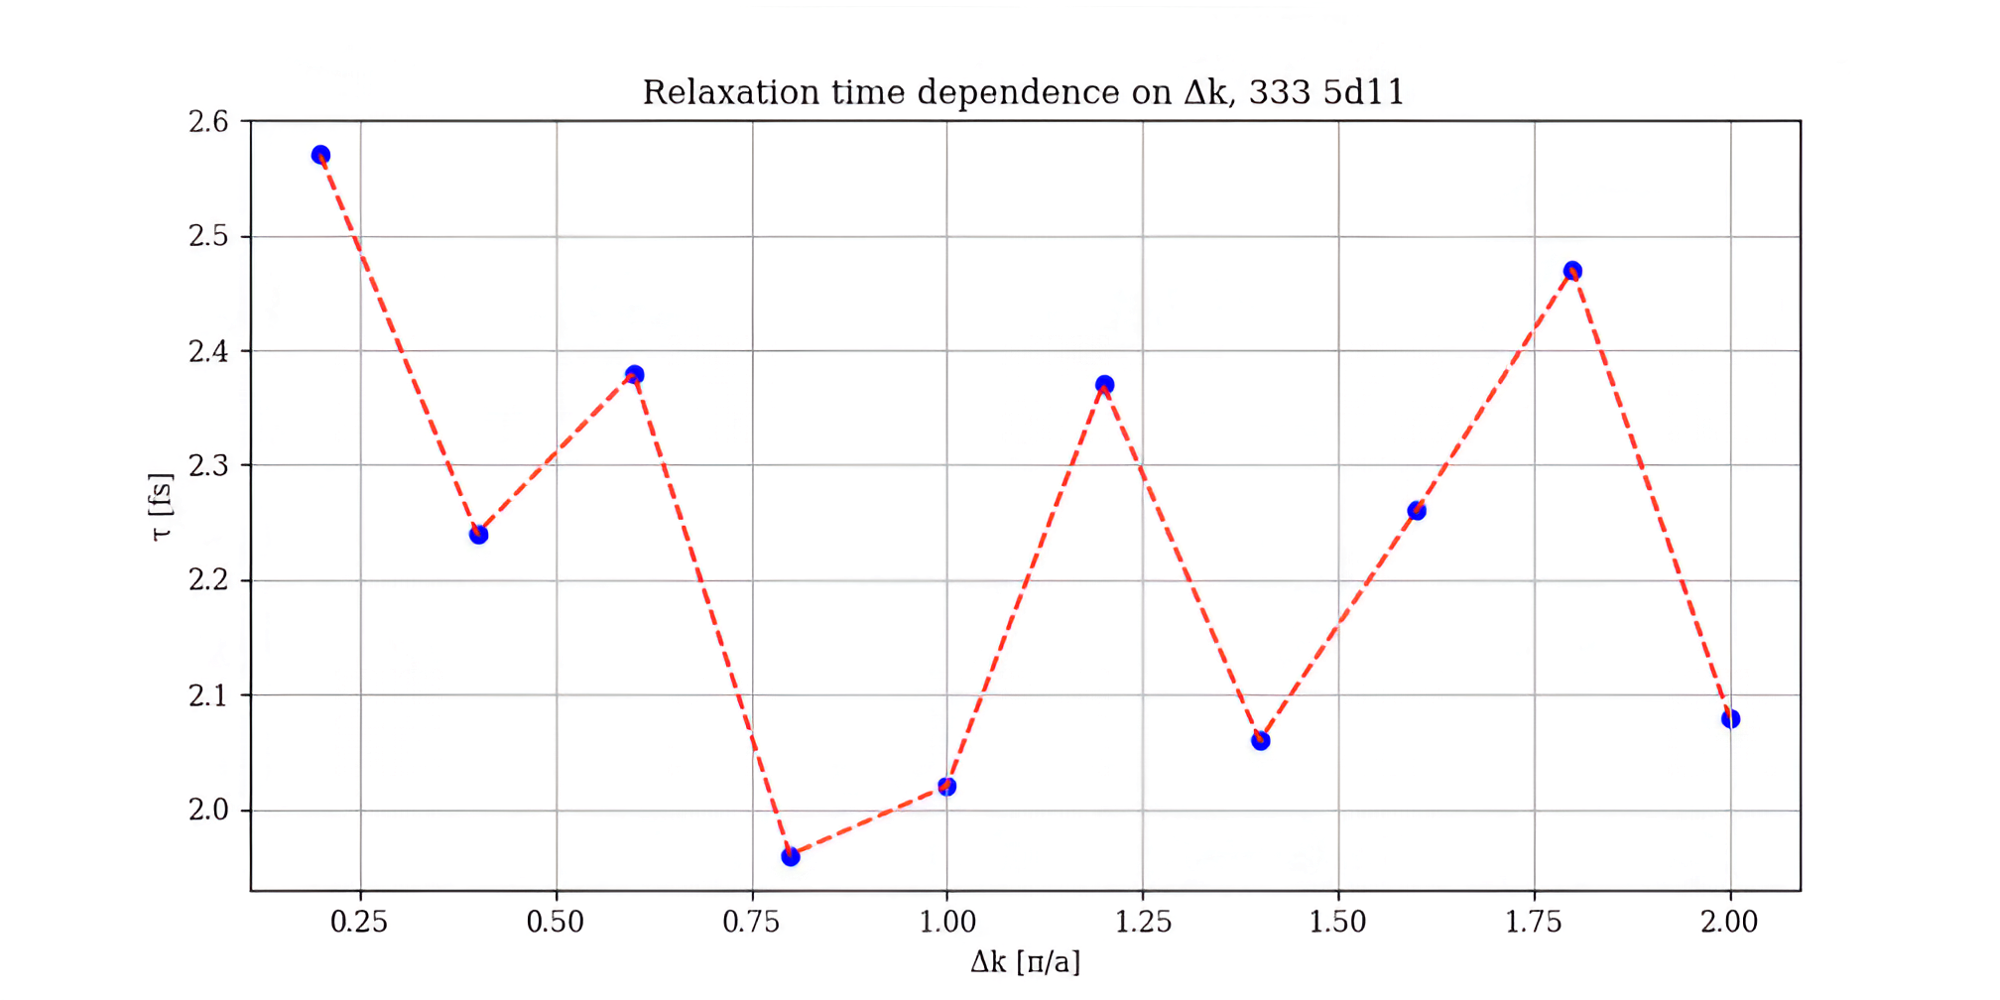
\includegraphics[width=0.6\linewidth]{figures/relaxation_k_dependence_v1.png} % путь к файлу
    \caption{Relaxation time dependence on wave vector.}
    \label{fig:myimage}
\end{figure}


Our pumping parameters are such (we need to verify this) that the gamma point of the conduction band is populated. Scattering theory predicts that for disorder in the form of random displacements of atoms from their equilibrium positions, the relaxation time should decrease as the wave vector increases, which is what we observe up to a certain point. The parabolic dispersion model quickly begins to fail, as can be seen from the silicon band structure. Parabolicity persists for only 10-20\% of the Brillouin zone (distance to L-point equals $\pi/a \sqrt{3}$). We could try the Kane model, which takes nonparabolicity into account.




The Kane model describes the nonparabolic energy dispersion in narrow–gap
semiconductors by introducing a correction to the parabolic band structure.
For the conduction band, the energy--momentum relation takes the form
\begin{equation}
E\,(1 + \alpha E) = \frac{\hbar^{2} k^{2}}{2 m^{\ast}},
\label{eq:kane}
\end{equation}
where $\alpha$ is the nonparabolicity parameter (typically
$\alpha \sim 1/E_{g}$), $m^{\ast}$ is the band-edge effective mass, and
$E$ is the carrier kinetic energy.




Solving Eq.~\eqref{eq:kane} for $E(k)$ yields
\begin{equation}
E(k) = \frac{1}{2\alpha}
\left[
\sqrt{1 + 2 \alpha \frac{\hbar^{2} k^{2}}{m^{\ast}}}
- 1
\right].
\end{equation}



The energy-dependent effective mass follows as
\begin{equation}
m(E) = m^{\ast} (1 + 2\alpha E).
\end{equation}

In scattering theory, the velocity and density of states must be modified.
The group velocity becomes
\begin{equation}
v(E) = \frac{1}{\hbar} \frac{\partial E}{\partial k}
     = \sqrt{\frac{2E(1+\alpha E)}{m^{\ast}}}\, \frac{1 + 2\alpha E}{1 + \alpha E},
\end{equation}
and the 3D density of states takes the form
\begin{equation}
g(E) = \frac{1}{2\pi^{2}}
\left( \frac{2 m^{\ast}}{\hbar^{2}} \right)^{3/2}
\sqrt{E(1+\alpha E)}\, (1 + 2\alpha E).
\end{equation}

These modifications must be used in calculating scattering rates, mobility,
and transport coefficients when nonparabolicity is significant.



\section{Gabor Transform}

\textcolor{red}{TO DO}
